\documentclass{article}
\usepackage{graphicx}
\usepackage{float}
\usepackage{subcaption}
\title{Studio della legge oraria di un corpo in caduta libera}
\author{Alessandro Di Meglio\\Francesco Angelo Fabiano Antonacci}

\date{\today}

\begin{document}

\maketitle

\section{Scopo dell'esperienza}
Lo scopo dell’esperienza è lo studio della legge oraria di un corpo in caduta libera.

\section {Cenni Teorici}
Il moto di un corpo uniformemente accelerato è dato dalla seguente equazione:

\begin{equation}
h(t)=\frac{1}{2}at^2+v_0t+h_0
\label{fond}
\end{equation}



\section{Apparato sperimentale}
\subsection{Strumenti di acquisizione}
Lo strumento di acquisizione è stata la fotocamera di uno smartphone che riprende a 960 fps.

\subsection{Grave}
Il grave con cui è stato deciso di effettuare l'esperimento è una sfera di acciaio di 8 millimetri di diametro.

\subsection{Strumenti di calibrazione}
Sono stati usati un filo a piombo e un metro a nastro con una risoluzione di 1 mm.
Il metro a nastro è stato utile per riscalare i dati presi in pixel dai frame.

\section{Descrizione delle misure}
E' stato disposto verticalmente il metro a nastro grazie al filo a piombo per segnare una verticale.
E' stato registrato un filmato a rallentatore con lo smartphone per aumentare la messa a fuoco del corpo in movimento.
Successivamente sono stati estratti dei frames a intervalli regolari di tempo.
Sono state prese delle distanze in pixel sulla verticale con un medesimo punto di riferimento.

\subsection{Incertezza sui tempi}
Come incertezza sui tempi si è preso il 0.001 secondi:ossia il tempo che divide due frame consecutivi.

\subsection{Incertezza sulle posizioni}
Come incertezza sulle posizioni è stata presa la metà della lunghezza della sagoma del corpo per ciascun frame.
Si osserva che l'incertezza cresce proporzionalmente ai tempi in quanto essa è determinata dalla velocità, la quale cresce approssimativamente proporzionalmente al tempo.

\section {Analisi dei dati}

Per utilizzare l'algoritmo di best fit curve\_fit() per l'equazione (\ref{fond}) è stata verificata la seguente relazione:

\begin{equation}
\sigma x\gg\left|\frac{dx}{dt}\right|\sigma t
\end{equation}
Si trova che il termine a sinistra è sempre molto maggiore di quello a destra: nel caso estremo in cui si paragonano tra loro la velocità massima e l'incertezza più piccola sulla distanza la relazione è valida comunque, pertanto la relazione è verificata per ogni istante.

L'algoritmo di best fit restituisce i seguenti valori:

\begin{center}
  \begin{tabular}{|c|c|c|}
    \hline
	$\hat{a} $[m/$s^2$] &  $ \hat{v_0} $ [m/s] & $ \hat{c_0}$ [m] \\
    \hline
	$-9.8\pm0.2$ & $-0.7\pm0.05$& $2.16\pm0.01$\\
   \hline
  \end{tabular}
\end{center}


\begin{figure}
	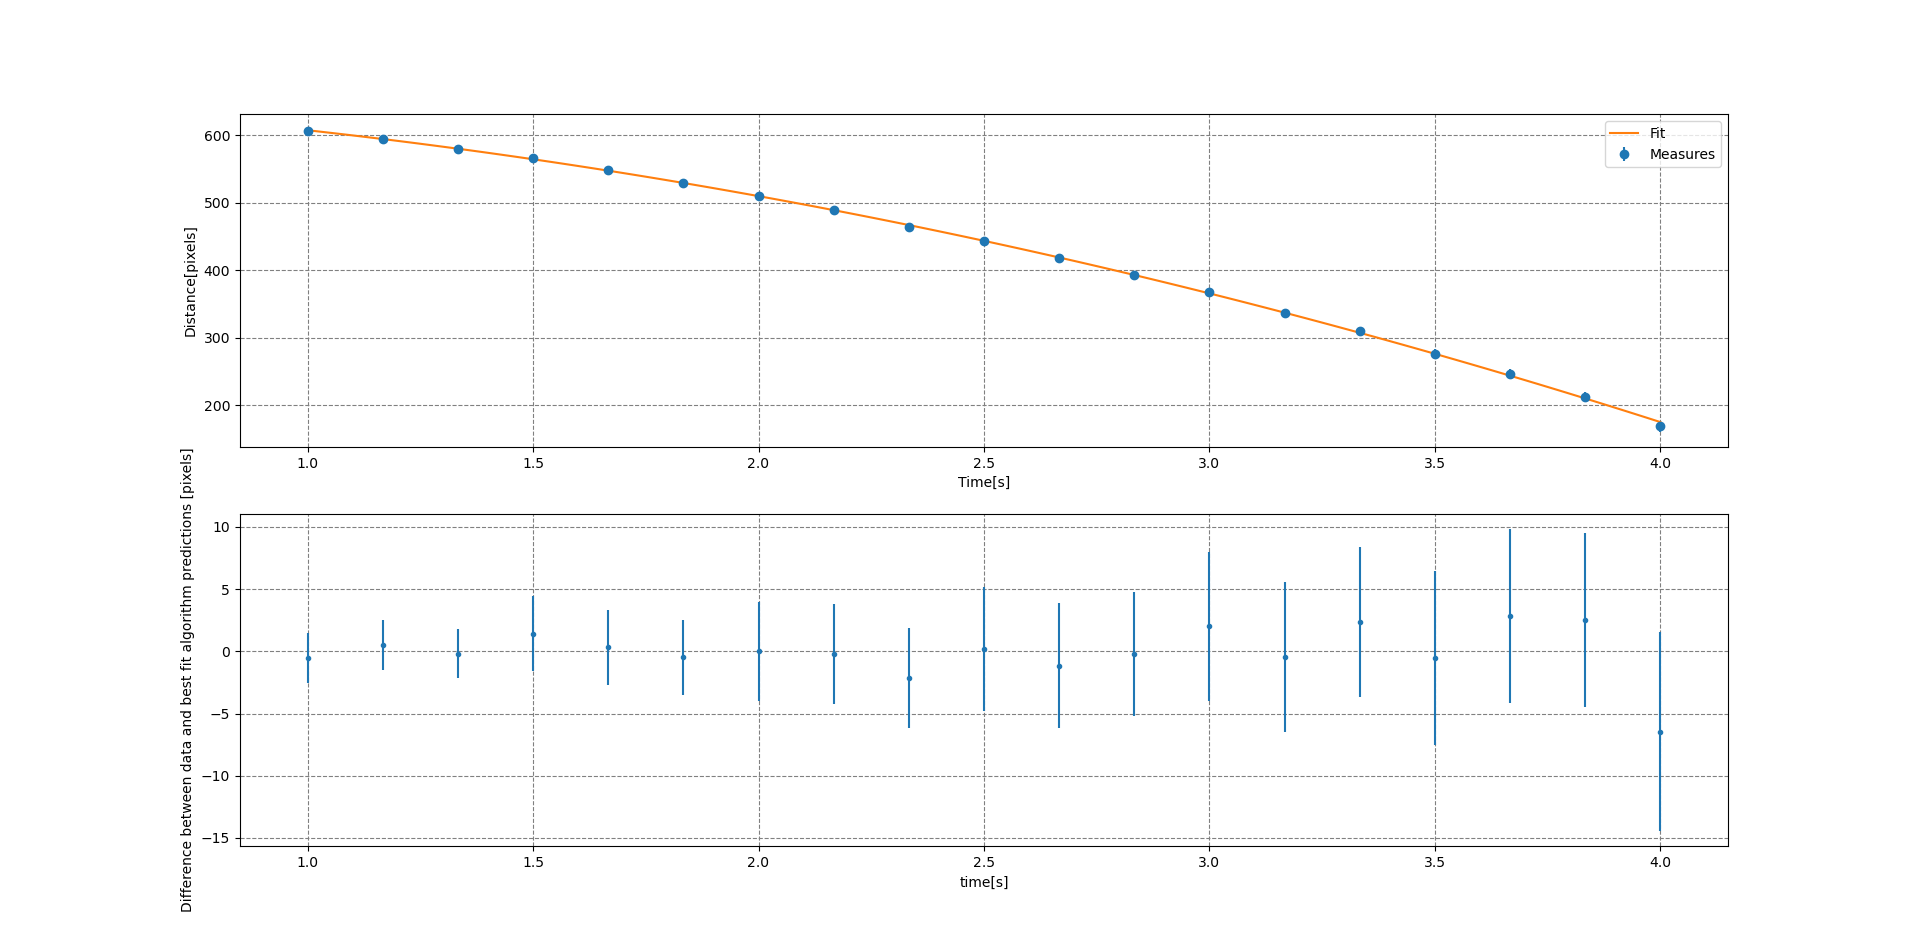
\includegraphics[width=\textwidth]{Falling_mass_plot.png}
\end{figure}

\section{Conclusione}
Dal grafico dei residui si osserva che tutte le misure si trovano a meno di una barra di errore dal fit: il modello dell'equazione (\ref{fond}) è buono.
Il valore calcolato dell'accelerazione di gravità è $g= 9.8\pm 0.2 $[m/$s^{-2}$].


\end{document}

\end{document}
